
\documentclass{article}

\usepackage[margin=1in]{geometry} 
\usepackage[french]{babel}
\usepackage[T1]{fontenc}
\usepackage[utf8]{inputenc}
\usepackage{amsmath,amsthm,amssymb,amsfonts, fancyhdr, color, comment, graphicx, environ}
\usepackage{xcolor}
\usepackage{mdframed}
\usepackage[shortlabels]{enumitem}
\usepackage{indentfirst}
\usepackage{hyperref}
\usepackage{lastpage}
\usepackage{listingsutf8}
%\usepackage{ff++listings}
\usepackage{amsmath}
\DeclareMathOperator{\Tr}{Tr}

\usepackage{physics}
\usepackage{amsfonts}
\usepackage{float}
\PassOptionsToPackage{hyphens}{url}\usepackage{hyperref}

\usepackage{xurl}

\renewcommand{\footrulewidth}{0.8pt}
\hypersetup{
    colorlinks=true,
    linkcolor=blue,
    filecolor=magenta,      
    urlcolor=blue,
}

\pagestyle{fancy}

\newenvironment{problem}[2][Etape]
    { \begin{mdframed}[backgroundcolor=gray!20] \textbf{#1 #2} \\}
    {  \end{mdframed}}

\newenvironment{solution}{\textbf{Réponse}}

\lhead{L. Gomes et F. Pollet}
\rhead{ES Elements finis} 
\chead{\textbf{Optimisation de l'épaisseur d'un pont}}
\lfoot{D. Ryckelynck, N. Spillane, P.-H. Tournier}
\cfoot{Mines Paris}
\rfoot{\thepage/\pageref*{LastPage}}


\begin{document}

    \title{\Large ES Elements Finis  \\[0.5cm]
        \bf\Large Optimisation de l'épaisseur d'une structure tridimensionnelle}
\author{\large Leticia Gomes\\Pollet Florent \ \\}
\date{\large\today}

\makeatletter
    \begin{titlepage}
        \begin{center}
	   { 
\includegraphics[width=12cm]{mp_logo.png}}
	   {\ \\ \ \\}
        \vbox{}\vspace{5cm}
            {\@title }\\[3cm] 
            {\@author}
            {\large \ \\ Encadrants: \bf David Ryckelynck, Nicole Spillane et Pierre-Henri Tournier\\ \ \\}
            {\@date\\}

        \end{center}
    \end{titlepage}

    \tableofcontents

    \clearpage
\makeatother%not necessary but looks fancy

    % rappel du problème ? reprendre photo du sujet
    % référence à la fin
    % appendix pour code ?

    \section{Présentation du problème}
    La méthode des éléments finis est une méthode matématique utilisée par industriels et chercheurs afin de résudre numériquement des équations aux dérivées partielles. Une application envisageable pour les calculs avec la méthode des éléments finis est l'optimisation de l'épaisseur d'une structure tridimensionelle, 
    qui est ainsi l'objectif de ce projet. 
    La structure tridimensionnelle choisie est un pont pour lequel nous avons cherché à minimiser l'épaisseur
    en respectant une contrainte de déplacement vertical maximal en son centre de $10$ cm malgré l'application d'une force surfacique
    constante sur la surface horizontale supérieure du pont. 
    La géométrie de ce problème est tridimensionnelle et sa coupe verticale est montré dans la Figure \ref{fig:problem}.
    \begin{figure}[H]        
    \begin{center}
	
        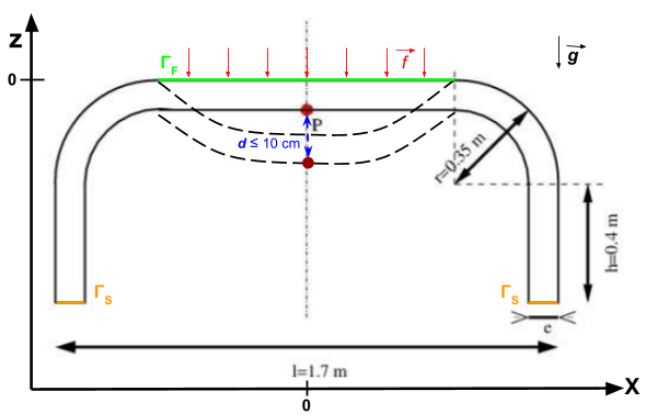
\includegraphics[width=12cm]{coupe_2D-schema.JPG}
        \caption{Schéma de la géométrie du pont. Une force surfacique $f= - 5x10^8 N m^(-2)$ est appliquée à sa surface supérieure. Le déplacement maximale $d$ est montré en bleue, en vert c'est $\gamma$F, surface dans lequelle la force est appliquée et $\gamma$S est la surface inférieure fixe. Le système est qui est soumis à la gravité $g$.}
        \label{fig:problem}
    
	\end{center}
    \end{figure}
    
    La structure est considérée comme homogène avec les extrémités inférieures fixes et une largeur $p = 0,5 m$. 
    
    Les données fournis pour ce système sont :
    
    \begin{itemize}
    \item Module d'Young : $E = 2.1 \times 10^11$ N m$^{-2}$
    \item Coefficient de Poisson : $\nu = 0.3$ 
    \item Masse Volumique : $\rho = 7800$ kg m$^{-3}$
    \item Force imposée sur le bord supérieur : $f= - 5 \times 10^8$ N m$^{-2}$
    \end{itemize}
    
    Nous avons adopté la stratégie suivante pour traiter ce projet, en trois parties :
    \begin{enumerate}
        \item Établissement de la formulation variationelle pour ce problème ;
        \item Résolution à épaisseur fixée : nous avons écrit un programme avec la langage FreeFem++ pour résoudre le système à épaisseur fixe $e = 0,1 m$, 
            avec une maille initialement bidimentionelle qui est ensuite complétée avec la fonction $buildlayers$. 
            Nous avons étudié la différence entre des solutions calculées pour la pièce et pour sa moitié ainsi que la précision du résultat en variant le maillage.
        \item Optimisation de l'épaisseur :
        \begin{enumerate}
            \item Approximation graphique : 
                nous avons analysé la relation entre l'épaisseur et le déplacement afin de trouver un intervalle où le déplacement est inférieur ou égal à 10 cm.
            \item Raffinement de la solution : nous avons utilisé la méthode de dichotomie pour résoudre le système.
        \end{enumerate}
    \end{enumerate}

    \newpage
    
    \section{Formulation variationnelle}

    \begin{problem}{1}
    Mettons le problème sous forme faible (variationnelle) pour pouvoir le résoudre avec la méthode des éléments finis.
    \end{problem}
    
    \begin{solution}   
        On part de la formulation forte. On cherche le déplacement $\vec{u}$, fonction de $\mathbb{R}^3$ dans $\mathbb{R}^3$.

Pour cela, on réalise d'abord un bilan des forces sur le système étudié qui est le pont dans le référentiel terrestre. Le système est à l'équilibre donc $\vec{a} = 0$.

On définit

\begin{equation}
    \vec{f} = \begin{pmatrix} 0\\ 0\\ f\\\end{pmatrix}
\end{equation}

et sa valeur est spécifiée dans l'énoncé.

On définit 

\begin{equation}
    \vec{g} = \begin{pmatrix} 0\\ 0\\ -g\\\end{pmatrix}
\end{equation}

où $g$ est l'accélération de la pesanteur standard.

On se place en 3D. On définit le domaine $\Omega$ comme l'ensemble du pont (qui est un polygone), et la frontière $\Gamma$ est partitionnée comme selon le schéma.

Le schéma n'est pas à l'échelle.

D'après le cours de mécanique,

\begin{equation}
    \begin{cases}
        \lambda = \frac{E}{2(1+\nu)}\\
        \mu = \frac{\nu E}{(1+\nu)(1-2\nu)}
    \end{cases}
\end{equation}

et on cherche donc $\vec{u} \in \mathcal{C}^2(\bar{\Omega})^3$ tel que

\begin{equation}\label{fort}
    \begin{cases}
      \div \sigma + \rho \vec{g} = 0 \textrm { sur $\Omega$ (première loi de Cauchy)} \\
      \sigma = \lambda \Tr (\varepsilon) I + 2 \mu \varepsilon \textrm { (loi de comportement en élasticité linéaire)} \\
      \varepsilon=\frac{\nabla u + \nabla u^T }{2} \textrm { (compatibilité)} \\
      \sigma \cdot \vec{n} = \vec{f}\textrm { sur $\Gamma_F$ (condition de Neumann)} \\
      \sigma \cdot \vec{n} = 0\textrm { sur $\Gamma \backslash (\Gamma_F \cup \Gamma_S) $ (condition de Neumann)} \\
      \vec{u} = 0 \textrm { sur $\Gamma_S$ (condition de Dirichlet)} \\
      
    \end{cases}
\end{equation}

On a bien les conditions de continuité et de différentiabilité souhaitées. %à prouver, problème un peu différent%

Etant donné que l'on a dans le cours uniquement des formules pour des inconnues scalaires, on va écrire les équations pour chaque coordonnée pour arriver à la formulation variationnelle.

On note $\sigma_i$ la transposée de la $i$-ème ligne du $\sigma$.

Considérons une solution du problème.
Soit $i \in \{1,2,3\}$.
Soit $v_i \in \mathcal{C}^1(\bar{\Omega})$ tel que $v_{i|\Gamma_S} = 0$.
% def sigma
% def v


La première équation de \eqref{fort} se réécrit 
$$\div \vec{\sigma_i} + \rho g_i = 0$$
On multiplie par $v_i$ et on intègre sur $\Omega$ :
$$\int_\Omega v_i \div \vec{\sigma_i} +  \int_\Omega v_i \rho g_i = 0$$

On réalise une intégration par partie selon la formule de Green, car $\vec{\sigma_i} \in \mathcal{C}^1(\bar{\Omega})^3$ et $v_i \in \mathcal{C}^1(\bar{\Omega})$ :


\begin{equation}\label{green}
    -\int_{\Omega} \vec{\sigma_i} \cdot \grad v_i + \int_{\Gamma} v_i (\vec{\sigma_i} \cdot \vec{n}) + \int_\Omega v_i \rho g_i = 0
\end{equation}

On injecte les conditions de Neumann et de Dirichlet dans l'équation : %+conditions de dirichlet 

\begin{equation}
    \begin{cases}
        -\displaystyle\int_{\Omega} \vec{\sigma_i} \cdot \grad v_i + \int_{\Gamma_F} v_i f_i + \int_\Omega v_i \rho g_i = 0\\
        u_i = 0 \textrm{ sur } \Gamma_S
    \end{cases}
\end{equation}

Sommons maintenant les trois équations pour chaque $i \in \{1,2,3\}$.

En utilisant la convention de sommation d'Einstein (les indices répétés sont sommés, de $1$ à $3$), on remarque que :
$$
\vec{\sigma_i} \cdot \grad v_i = \sigma_{ij} \frac{\partial v_i}{\partial x_j}
$$
puis que, en notant $\delta$ le symbole de Kronecker et en utilisant les propriétés de la trace :
$$
\sigma_{ij} = \lambda \Tr(\grad \vec{u}) \delta_{ji} + \mu (\frac{\partial u_i}{\partial x_j} + \frac{\partial u_j}{\partial x_i})
$$

On utilise le fait que $\Tr(\grad \vec{u}) = \div \vec{u}$ pour arriver à 

$$
\vec{\sigma_i} \cdot \grad v_i = \lambda \div \vec{u} \div \vec{v} + \mu (\frac{\partial u_i}{\partial x_j} + \frac{\partial u_j}{\partial x_i})\frac{\partial v_i}{\partial x_j}
$$
%(\delta_{ji} \frac{\partial v_i}{\partial x_j}) 

On définit :

$$
\epsilon(\vec{x})=
\begin{pmatrix}
    \partial_1 x_1\\
    \partial_2 x_2\\ 
    \partial_3 x_3\\
    \frac{1}{\sqrt{2}}(\partial_3 x_2 + \partial_2 x_3)\\
    \frac{1}{\sqrt{2}}(\partial_3 x_1 + \partial_1 x_3)\\
    \frac{1}{\sqrt{2}}(\partial_2 x_1 + \partial_1 x_3)\\
\end{pmatrix}
$$

On constate enfin, en développant, que :
$$
(\frac{\partial u_i}{\partial x_j} + \frac{\partial u_j}{\partial x_i})\frac{\partial v_i}{\partial x_j} = 2\epsilon(\vec{u})\epsilon(\vec{v})
$$

On arrive donc au problème suivant  :

Trouver $\vec{u} \in \mathcal{C}^2(\bar{\Omega})^3$ tel que
\begin{equation}\label{varia}
    \begin{cases}
        \displaystyle\int_{\Omega} (\lambda \div \vec{u} \div \vec{v} + 2\mu \epsilon(\vec{u})^T \epsilon(\vec{v})) - \int_{\Gamma_F} \vec{v} \cdot \vec{f} - \int_\Omega \rho \vec{v} \cdot \vec{g} = 0 \textrm{ } \forall \vec{v} \in \mathcal{C}^1(\bar{\Omega})^3\\
        \vec{u} = 0 \textrm{ sur } \Gamma_S
    \end{cases}
\end{equation}


    \end{solution}

    \section{Résolution à épaisseur fixée}

    \section{Optimisation de l'épaisseur}

    \subsection{Approximation graphique}
    \subsection{Raffinement de la solution}
    Afin d'utiliser la méthode dichotomie, nous avons défini des variables $e^n_{min}$ et $e^n_{max}$  qui seront utilisé pour calculer une épaisseur moyenne $e^n$ 	qui donnera le déplacement $d^n$. Si:
    \begin{itemize}
    \item $|d^n| <= |d_0|$, la valeur moyenne $e^n$ sera la nouvelle valeur de $e^n_{max}$ et $e^n_{min}$ reste constante.
    \item $|d^n| >= |d_0|$, la valeur moyenne $e^n$ sera la nouvelle valeur de $e^n_{min}$ et $e^n_{max}$ reste constante.
    \end{itemize}
    À partir du graph \ref{...} généré dans la section précédente, nous avons choisit des valeurs initiales pour $e^n_{min}$ et $e^n_{max}$ de 10 cm et 30 cm respectivement. Après les calculs, les valeurs obtenues sont:
    \begin{center}
    $d_n = - 0,0999397 m$
    $e_n = 0,1531125 m$
    \end{center}
    
    \clearpage
    \appendix
    \section {Code source}

    Disponible sur ...

    \lstinputlisting[language=FreeFem]{simulation-v2.edp}


    %code + lien github
    
\end{document}
